\documentclass[11pt]{article}
\usepackage{geometry}                
\geometry{letterpaper}                   
\usepackage{graphicx}
\usepackage{subfigure}
\usepackage{subfig}
\usepackage{amssymb}
\usepackage{epstopdf}
\usepackage{abstract}
%\usepackage{natbib}
\usepackage{amssymb, amsmath}
\usepackage{algorithm}
\usepackage[noend]{algpseudocode}
%\usepackage{cite}

%
\makeatletter
\setlength{\@fptop}{0pt}
\makeatother
%


\DeclareGraphicsRule{.tif}{png}{.png}{`convert #1 `dirname #1`/`basename #1 .tif`.png}

%\title{Robustness Analysis of Social Networks under Different Attack Models}
%\author{Name 1, Name 2, }
%\date{date} 

\begin{document}


\begin{document}
\thispagestyle{empty}


\begin{center}
%\includegraphics[width=5cm]{ETHlogo.eps}

\bigskip


\bigskip


\bigskip


\LARGE{ 	Lecture with Computer Exercises:\\ }
\LARGE{ Modelling and Simulating Social Systems with MATLAB\\}

\bigskip

\bigskip

\small{Project Report}\\

\bigskip

\bigskip

\bigskip

\bigskip


\begin{tabular}{|c|}
\hline
\\
\textbf{\LARGE{Robustness Analysis of Social Networks}}\\
\textbf{\LARGE{under Different Attack Models}}\\
\\
\hline
\end{tabular}
\bigskip

\bigskip

\bigskip

\LARGE{Ghosh, Partha \& Thapa, Manish Jung \& Acharya, Dinesh}



\bigskip

\bigskip

\bigskip

\bigskip

\bigskip

\bigskip

\bigskip

\bigskip

Zurich\\
May 2015\\

\end{center}



\newpage

%%%%%%%%%%%%%%%%%%%%%%%%%%%%%%%%%%%%%%%%%%%%%%%%%

\newpage
\section*{Agreement for free-download}
\bigskip


\bigskip

\large We hereby agree to make our source code for this project freely available for download from the web pages of the SOMS chair. Furthermore, we assure that all source code is written by ourselves and is not violating any copyright restrictions.

\begin{center}

\bigskip


\bigskip

\bigskip

\begin{tabular}{@{}p{1cm}@{}p{5cm}@{}@{}p{5cm}@{}@{}p{5cm}}
\begin{minipage}{0cm}

\end{minipage}
&
\begin{minipage}{6cm}
\large Acharya, Dinesh

 %\vspace{\baselineskip}

\end{minipage}
&
\begin{minipage}{6cm}

\large Ghosh, Partha

\end{minipage}
&
\begin{minipage}{6cm}

\large Thapa, Manish Jung

\end{minipage}
\end{tabular}


\end{center}
\newpage

%%%%%%%%%%%%%%%%%%%%%%%%%%%%%%%%%%%%%%%



% IMPORTANT
% you MUST include the ETH declaration of originality here; it is available for download on the course website or at http://www.ethz.ch/faculty/exams/plagiarism/index_EN; it can be printed as pdf and should be filled out in handwriting


%%%%%%%%%% Table of content %%%%%%%%%%%%%%%%%

\tableofcontents

\newpage

%%%%%%%%%%%%%%%%%%%%%%%%%%%%%%%%%%%%%%%

\begin{abstract}
This paper investigates cascading disaster spreading in a network under random attacks. Further, it targets at answering the questions of the degree of robustness of network under a single node failure. Disease spreading as an example of cascading disaster spreading is considered in this paper. Models like SIR have been used in the past to simulate disease spreading in a society. In this paper, a slightly more general model for disease spreading is used.  This model has more parameters to tune, and realistic scenarios that involves features like link delay time, graceful failure and disturbance propagation could be taken into the consideration. The goal is to create a weighted robustness metric that quantifies the severity of the disaster a network is likely to face under a single-node failure scenario. An exhaustive simulation experiments is run with the model to quantify the robustness of various small-world networks with different node-degree distribution. 

\end{abstract}
\clearpage

\section{Individual contributions}
Partha and Dinesh were responsible for coding the disaster-spreading differential equation. Manish's task was to run a series of simulation experiment using this differential equation for various kinds of networks. As will be discussed below, robustness of the  networks under single-node failure is investigated. 


\section{Introduction and Motivations}
We live in a connected world. Our cities with their trade and travel routes form a complicated web. Social networks on the other hand forms subtler but more intricate web of links. Naturally information, goods and services reach the end user by taking several hops and through several channels. Until recently we did not take a critical look at bearing capacity, routing and robustness of the established systems. Research also reveals that the network that has been created based mainly on supply-demand dynamics is not optimal in many aspects. One serious concern about any networked system is its robustness against random node failure. In a real life setting it could mean breakout of infectious disease or flow of information in a social networks. As can be imagined it is just matter of time before an otherwise benign abnormality lead to disastrous conditions, because of simple structural imperfections in a network, it is important to study structural robustness of different kinds of network. In our study we examine how different networked systems behave when nodes in then fail to respond properly. The real life analogy would be spread of disease from one city to another starting from one or more cities. We explore what kind of connection structure stand better chance in avoiding total failure.
\subsection{Literature Review}
Most of the disease models categorise the given population into different categories and model the evolution of number of population in each of those categories with a set of differential equations. The popular susceptible infectious recovered (SIR) model is modelled by following set of differential equations:
\[ \frac{dS}{dt} = bN - \lambda S - dS,  \]
\[ \frac{dI}{dt} = \lambda S - gI - dI, \]
\[ \frac{dR}{dt} = gI - dR. \]

where $N = S + R + I$ is the total population size, $\lambda$ is the rate at which infectious individuals become infected, $g$ is the rate of recovery from infection, $d$ is the natural death rate and $b$ is the birth rate. The SIR models the diseases where there is no chance of infection once infected such as in the case of measles. Another popular model is susceptible-infectious-susceptible $SIS$ model which is given by following set of differential equations:
\[ \frac{dS}{dt} = gI - \lambda S,  \]
\[ \frac{dI}{dt} = \lambda S - gI. \]

SIR model is used to model diseases where there are high chances of repeated infections such as in the case of STDs like Chlamydia.\\
\\
These standard models do not take into account the fact that pattern of interactions at individual level also play significant role in spread of disease. Standard Network Theoretic modelling of disease spread takes into account this factor by considering the network of individuals. Each individual is considered as a node and the possible interactions or contact between individuals is considered as a edge on the graph. The adjacency matrix $A$ is constructed such that $A_{ij} = 1$ if the disease can transfer from individual $i$ to individual $j$ and $0$ otherwise. The properties of the adjacency matrix can be studied to deduce about the structure of the network. To simulate disease spread in the network, different techniques has been used. One such model uses simple equation
\[ \text {rate of infection} = \tau \times n \] where n is number of infectious nodes in neighborhood, $\tau$ is transmission rate. This has been discussed in more details on \cite{keeling}.\\
\\
Similarly, the effect of structure of network on topology has been discussed in \cite{shirley}. There the authors use a probabilistic model to simulate the spread of disease in the network. At each step of simulation, a vertex was randomly picked. It then infects all of the neighbouring nodes with given probability of infection. The vertices remain infectious only for a certain latency period. After that, they are no more infectious and also immune to disease.

\subsection{Research Problem}
In this paper, we use a different differential equation to simulate the spread of disease in the network. We implement and discuss the cascading model by Lubos Buzna, et al. \cite{helbing} for disaster spread in its own terms, rather than spread of disease within a given population as in majority of related works, we look at spread of disease across cities in the whole world. So vertices represent cities rather than individuals in the given population.\\
\\
With such dynamics, disease spreading in a social network (like cities or countries) will be investigated.  Our analysis is based on N-1 node-failure analysis. Meaning, it will be investigated whether or not the system is robust under single node failure; here failure implies node being infected by a disease. This in turn is determined if the overall health of a node crosses a certain threshold. We have set this threshold as $0.5$ for the the simulation experiments. The goal of the project is to run $N-1$ contingency analysis with each of the nodes of the network attacked, for various kinds of artificial computer-generated small-world networks, with varying node-degrees among nodes.
\\

 The number of nodes that fail, under the attack of initial node, will be registered. The same will be done for all the nodes in the network. The result will be averaged out and normalized with the system size and threshold parameter $\theta$ of the network. This normalization renders the health threshold $\theta$ a dimensional less parameter and eases way of comparison between networks simulated with different thresholds. However as mentioned earlier we keep this parameter constant throughout our set of simulation experiments. Our simulations were done with artificial networks, and the result have been compared to see the robustness of these networks under N-1 attack model. As mentioned earlier, the aim of this project is to construct a weighted robustness metric for social networks, which can be used not-only in cascading disease spread but across many disciplines like gas flow network, electricity grids, information flow in social networks, etc. given the dynamics represented by the differential equation discussed in this paper is followed. In addition, the evolution of cascading failure will also be investigated in the project. In other words, number of nodes that fail in each iteration also will be recorded, and the evolution of failing nodes displayed for each iteration. Hence this project can be regarded as an effort to build a simulation environment that is based on a generic yet very powerful model to capture subtlety in behavior of the real system.

\section{Description of the Model}
In this section we shall summarize the model to simulate disturbance in an undirected/ bidirectional graph. It is of worth noting at this point that the model simulates flow of disturbance in a graph that has certain characteristics described in the rest of the paragraph, and hence is completely independent of the physical phenomenon being modeled in a particular use-case. In general, the properties assumed here is inspired by flow of faulty electric grid node but as will be apparent from the following discussion in absence of any domain specific information it is reasonable to assume such behavior. Further more the model provides suitable control parameters to reduce or even remove effect of individual features of the model. This improves the usability of the model further. The model works on a graph $G = (N, S)$, where $N$ represents the set of nodes and $S$ represents the set of edges. Now the edges in general can be considered as directed but since it is uncommon to have disturbance flowing in one direction in the systems we consider for the current work we consider edges that go in both directions. Each real system exhibits a natural resistance to challenges to certain extent, which has been captured in the model by a special threshold $\theta > 0$ and a node is considered infected/ disturbed when net accumulated disturbance in a node exceeds this threshold. Since disturbance coming into a node can sum up to arbitrary values we apply a sigmoid function as in Eq.\ref{SIGMOID}
\begin{equation}
\theta(y) = \frac{1-exp(-\alpha y)}{1+exp[-\alpha(y-\theta_i)]} 
\label{SIGMOID}
\end{equation}
 Where $\alpha$ specifies the stiffness parameter. This parameter can be set differently in our implementation letting the user the flexibility of modeling varying sensitivity of nodes. The model takes a connectivity matrix $M_{ij}$. This matrix specifies the strength of influence of one node on the other. In our case this matrix is a symmetric matrix and the elements in the main diagonal do not have any meaning. Any non zero entry in this matrix signifies a connection between two nodes and any negative value in this matrix signifies inverse relationship between connected nodes. Although inverse relationship is rare in real world disease spreading it is perfectly possible in case of information spreading hence the generality is required at this point. The model also takes a time delay matrix $T_{ij}$. This matrix models the amount of time required for the disturbance to flow from one node to the neighboring connected node. Entries in this matrix can only be non-negative if the corresponding entry in the connectivity matrix $M_{ij}$ is also non zero. A negative entry in this matrix is not allowed as that would render the whole system non causal and hence can not be simulated except in the steady state. The model calculates $f(O_j) = \frac{aO_j}{1+bO_j}$. It captures the explain away effect of a cause. In some use-cases it is not justified to use this feature, e.g. in case of disease spread simulation. In such cases the user can set $a=b\rightarrow\infty$. Finally the disturbance while the get transmitted to the receiving node from the transmitting node can gain or lose strength. To capture this dynamics the model takes another parameter $\beta_ij$, which scales the transmitted effect via an exponential function. With all these parameters in place we can write the model as in Eq.\ref{MAIN_MODEL}

\begin{equation}
\frac{dx_i}{dt} = -\frac{x_i}{\tau_i}+\Theta\left(\sum_{i\ne j}{\frac{M_{ij}x_j(t-t_{ij})}{f(O_j)}e^{-\beta_{ji}}}\right) 
\label{MAIN_MODEL}
\end{equation}
Now in some use-cases the scaling parameter $\beta_{ij}$ might not be a useful. One can easily set it to $0$ in such cases.
\section{Implementation}
Now with the mathematical formulation in place let us focus on implementation details that may prove rather important factor in the performance of the overall system. As can be seen the above equation has two parts, the self healing part and the incoming disturbance part. In order to ensure generality and yet maintain compactness of the code we need to take a modular approach. Although usage of classes are discouraged in Matlab, due to degraded execution speed, since our goal was to maintain re-usability of code we decided to use an object oriented programming style. To simulate any network we create two main objects, nodes and network. A node in our implementation is a class which holds all the parameter and functionality local to the node. So it holds the parameter $\alpha$ denoting its sensitivity to incoming disturbance, the parameter $\tau$ denoting its recovery rate. The parameters $a$ and $b$ denotes its capacity to spread disturbance to nodes connected to it should also be stored in per-node basis but in most of our applications used constant values we decided to keep them as global parameters that apply to all nodes. Most used methods in the node class are named as $runNode$ and $Sigmoid$. As the names suggest the first one calculates the change of health of the node in current time step. Since the second part in the RHS of Eq.\ref{MAIN_MODEL} can not be calculated without the knowledge about the connectivity matrix and time delay matrix the part inside the sigmoid function $\Theta$, is passed to tihs function from the $NetworkBase$ class in a variable named $effectFromNeighbours$. The network base class is responsible for keeping track of the structure of the network being simulated and it does so by keeping a list of all the nodes and a connectivity matrix and a time delay matrix on the node indices. This class provides a few convenience functions to create a connectivity matrices on the fly for quick tryouts and debugging. The main methods are $addNode$, $delete$, and $simulateNetwork$. Add and delete node helps create the network by adding nodes to the network. Connections are not established at this point, but should be done separately through the method $connectAstoBs$. Finally the $simulateNetwork$ method simulates the whole network for one discrete time step. It updates the health of all the nodes present at the point of time this method is called. To simulate the network for several time steps this method must be called in a loop. The main work flow of the program can be seen in the following pseudocode.

\begin{algorithm}
\caption{Main work-flow of disturbance propagation}\label{MAIN_PSEUDO_CODE}
\begin{algorithmic}[1]
\Procedure{MAIN}{}
	\Procedure{SetupConfigurationParams}{}
			\State \texttt{Set MaxSimulationTime, TimeStep, StoppingCriterion}
			\State \texttt{Load/Generate edge strength matrix}
			\State \texttt{Load/Generate time delay matrix}
			\State \texttt{Create a new network, add nodes and connect them}
	\EndProcedure
	\Procedure{RunMainSimulation}{}
		\While {\texttt{NOT(StoppingCriterion) \&\& \! NOT(maxSimulationTimeReached)}}
			\State \texttt{net = net.simulateNetwork(timeStep);}
			\State \texttt{Log health of interesting nodes or any other parameter}
		\EndWhile
	\EndProcedure
\EndProcedure
\end{algorithmic}
\end{algorithm}

\newpage
\section{Simulation Results and Discussion}
The network is called N-1 robust if the damage it encounters is not significant under single node failure (or infection).  To see this, a series of simulation experiments were performed using the disaster-spreading equation (2) under single node failures. A node is initially infected, and the disease spreading observed. The network is than restored to its original state, and another node is infected and the disease spreading observed again. This is repeated for all the nodes of the network exhaustively. In the end, an array of health of nodes of the network is received for each iteration step for each of the single node failure scenario. Each of these array form an element of the ensemble for analysis of the final robustness metric of the network. \\
\\
Figure 1 shows the different types of networks studied in this paper. Small world network was studied for different distribution of node-degrees. These network were computer-generated using Watts-Strogatz algorithm. Figure 2 shows the degree distribution for these networks. As the probability of edge rewiring among the nodes is increased, the network signifies more and more random network, with non-uniform degree distribution. For $\beta=0$, the network is a ring lattice, with very small shortest path between any two nodes, and it represents the ideal small world network. For larger $\beta$, the shortest path between any two nodes increases. Figure 3 shows the simulation result for these networks under the model in equation (2). As $\beta$ increases, the damage the network encounters decreases on average. This is particularly visible during the first iteration where the damage the network with smallest $\beta$ experiences is significantly higher than those with larger $\beta$. As can be observed, the evolution of average health of nodes reaches equilibrium after 16 iterations for each of these networks. 

\begin{figure}[!htb]
\centering
\subfigure[$\beta$=0]{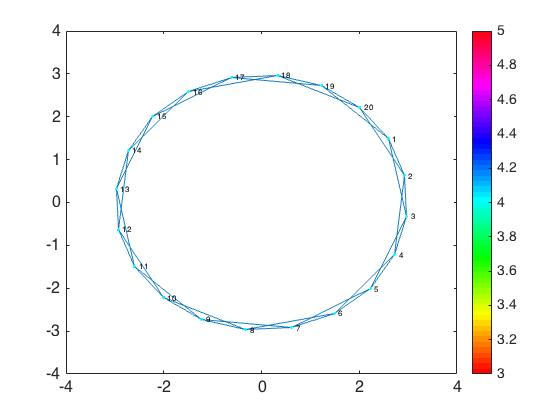
\includegraphics[width=0.49\columnwidth]{images/wattsona.jpg}}
\subfigure[$\beta$=0.15]{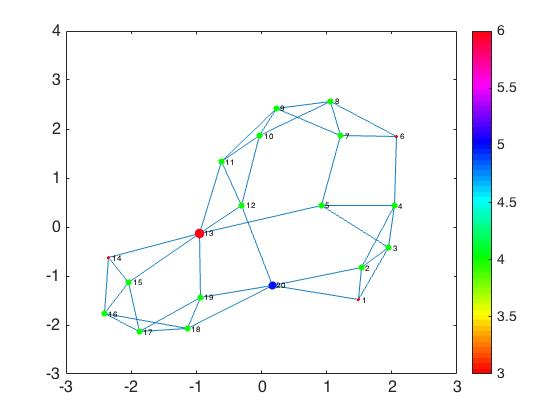
\includegraphics[width=0.49\columnwidth]{images/wattsonb.jpg}}
\subfigure[$\beta$=0.5]{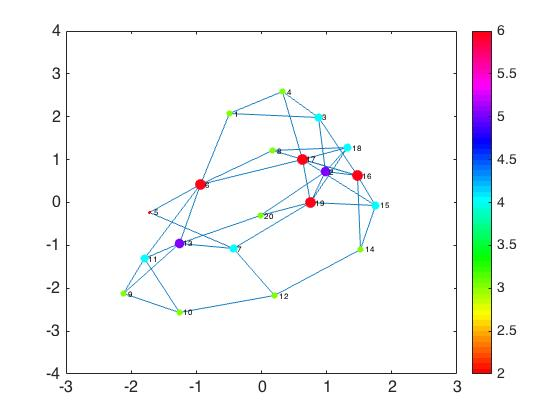
\includegraphics[width=0.49\columnwidth]{images/wattsonc.jpg}}
\subfigure[$\beta$=1]{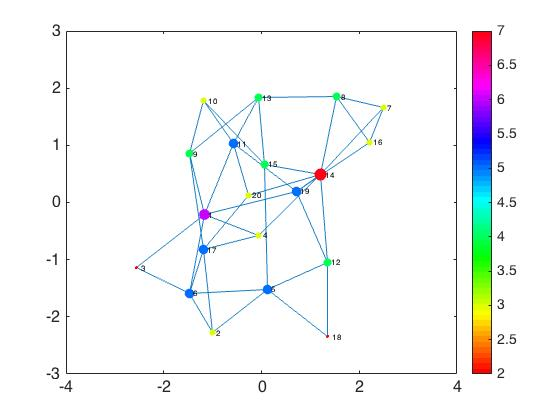
\includegraphics[width=0.49\columnwidth]{images/wattsond.jpg}}
\caption{Small world network constructed using Watts-Strogatz algorithm. The network size (N) and average node-degree (d) was fixed with N=20, and d=2, while the probability of rewiring ($\beta$) was gradually increased, making the network more and more random.}\label{fig:case-39-power-losses}
\end{figure}
\clearpage


\begin{figure}[!htb]
\centering
\subfigure[$\beta$=0]{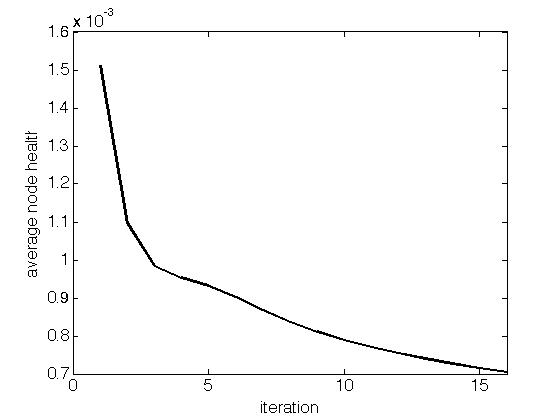
\includegraphics[width=0.49\columnwidth]{images/newbetaa.jpg}}
\subfigure[$\beta$=0.15]{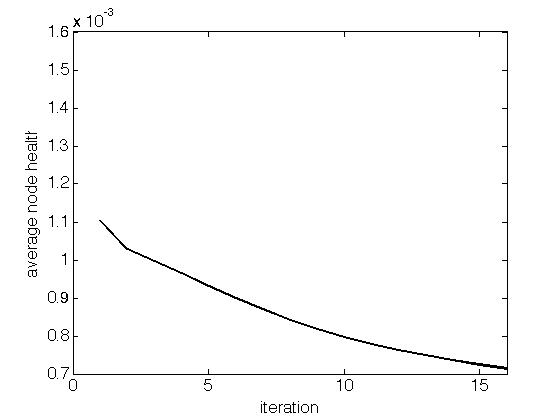
\includegraphics[width=0.49\columnwidth]{images/newbetab.jpg}}
\subfigure[$\beta$=0.5]{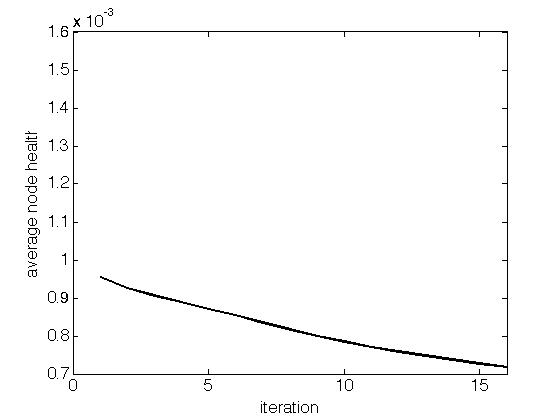
\includegraphics[width=0.49\columnwidth]{images/newbetac.jpg}}
\subfigure[$\beta$=1]{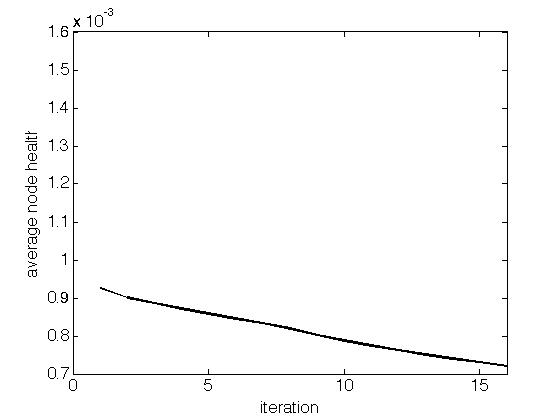
\includegraphics[width=0.49\columnwidth]{images/newbetad.jpg}}
\caption{Evolution of disease spread in each iteration step for different networks..}\label{fig:case-39-power-losses}
\end{figure}

Figure 4 shows the robustness metric under N-1 attack scenario for each of these networks. Each of this scatter point quantifies the robustness of the corresponding network; the smaller the average proportion infected per iteration the more robust is the network. The trend in the plot is quite clear. For smaller $\beta$, the less robust the network. 

\begin{figure}[t!]
\centering
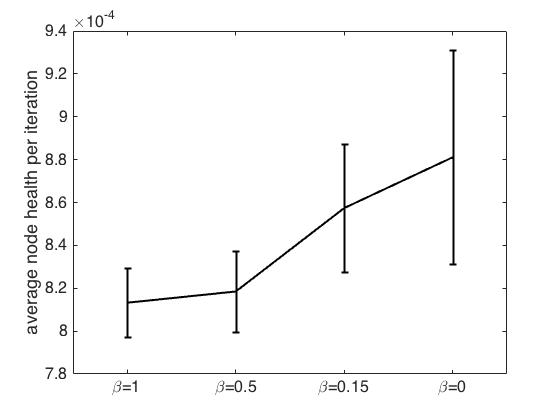
\includegraphics[width=0.70\columnwidth]{images/periteration.jpg}
\caption{Robustness metric for different $\beta$}
\end{figure}
\clearpage

\section{Summary and Outlook}
This paper confirms the smaller is the $\beta$ parameter of the small-world network under Watts-Strogatz model, the less robust is the network. This should not come as a surprise to us since smaller beta parameter means, the network exhibits strong long-range interaction between any two nodes. In other words, as discussed in the previous section, the average path length between any two nodes decreases for smaller $\beta$ parameter. The robustness tool that is presented in this paper will greatly aid future studies on trial-and-error optimization of network serviceability under cascading disaster spreading. Since the robustness metric, is based on ensemble averaging, and is ultimately quantified by a single real number, it comes with a great ease to study, and mitigate the cascading disaster spreading. Besides, the robustness metric presented here is fully a weighted one, given that actual simulation experiments is run to generate it. In addition, this tool will also aid the study of cascading-disaster spreading in other domains like water flow, electricity flow, gas flow or any-network that can potentially experience cascading failure.



\newpage
\begin{thebibliography}{9}
\bibitem{shirley} Shirley, Mark D.F. and Rushton, Steve P. \textit{ The impacts of network topology on disease spread }, Ecological Complexity, 2005.

\bibitem{helbing} Buzna, Lubos; Peters, Karsten; Ammoser, Hendrik;  Kuhnert, Christian and Helbing, Dirk.\textit{ Efficient Response to Cascading Disaster Spreading } .

\bibitem{keeling}
Keeling, Matt J. and Ken T.D. Eames. \textit{ Networks and Epidemic Models } Journal of the Royal Society Interface 2.4 (2005): 295–307. PMC. Web. 7 Dec. 2015.

\end{thebibliography}

\end{document}